\documentclass[]{article}
\usepackage{lmodern}
\usepackage{amssymb,amsmath}
\usepackage{ifxetex,ifluatex}
\usepackage{fixltx2e} % provides \textsubscript
\ifnum 0\ifxetex 1\fi\ifluatex 1\fi=0 % if pdftex
  \usepackage[T1]{fontenc}
  \usepackage[utf8]{inputenc}
\else % if luatex or xelatex
  \ifxetex
    \usepackage{mathspec}
  \else
    \usepackage{fontspec}
  \fi
  \defaultfontfeatures{Ligatures=TeX,Scale=MatchLowercase}
\fi
% use upquote if available, for straight quotes in verbatim environments
\IfFileExists{upquote.sty}{\usepackage{upquote}}{}
% use microtype if available
\IfFileExists{microtype.sty}{%
\usepackage{microtype}
\UseMicrotypeSet[protrusion]{basicmath} % disable protrusion for tt fonts
}{}
\usepackage[margin=1in]{geometry}
\usepackage{hyperref}
\hypersetup{unicode=true,
            pdftitle={VDA - Sommesemster 2019 - Visualisierungen der Suicide Daten von 1985-2016},
            pdfauthor={Philipp Dalheimer, Thomas Jäger},
            pdfborder={0 0 0},
            breaklinks=true}
\urlstyle{same}  % don't use monospace font for urls
\usepackage{color}
\usepackage{fancyvrb}
\newcommand{\VerbBar}{|}
\newcommand{\VERB}{\Verb[commandchars=\\\{\}]}
\DefineVerbatimEnvironment{Highlighting}{Verbatim}{commandchars=\\\{\}}
% Add ',fontsize=\small' for more characters per line
\usepackage{framed}
\definecolor{shadecolor}{RGB}{248,248,248}
\newenvironment{Shaded}{\begin{snugshade}}{\end{snugshade}}
\newcommand{\AlertTok}[1]{\textcolor[rgb]{0.94,0.16,0.16}{#1}}
\newcommand{\AnnotationTok}[1]{\textcolor[rgb]{0.56,0.35,0.01}{\textbf{\textit{#1}}}}
\newcommand{\AttributeTok}[1]{\textcolor[rgb]{0.77,0.63,0.00}{#1}}
\newcommand{\BaseNTok}[1]{\textcolor[rgb]{0.00,0.00,0.81}{#1}}
\newcommand{\BuiltInTok}[1]{#1}
\newcommand{\CharTok}[1]{\textcolor[rgb]{0.31,0.60,0.02}{#1}}
\newcommand{\CommentTok}[1]{\textcolor[rgb]{0.56,0.35,0.01}{\textit{#1}}}
\newcommand{\CommentVarTok}[1]{\textcolor[rgb]{0.56,0.35,0.01}{\textbf{\textit{#1}}}}
\newcommand{\ConstantTok}[1]{\textcolor[rgb]{0.00,0.00,0.00}{#1}}
\newcommand{\ControlFlowTok}[1]{\textcolor[rgb]{0.13,0.29,0.53}{\textbf{#1}}}
\newcommand{\DataTypeTok}[1]{\textcolor[rgb]{0.13,0.29,0.53}{#1}}
\newcommand{\DecValTok}[1]{\textcolor[rgb]{0.00,0.00,0.81}{#1}}
\newcommand{\DocumentationTok}[1]{\textcolor[rgb]{0.56,0.35,0.01}{\textbf{\textit{#1}}}}
\newcommand{\ErrorTok}[1]{\textcolor[rgb]{0.64,0.00,0.00}{\textbf{#1}}}
\newcommand{\ExtensionTok}[1]{#1}
\newcommand{\FloatTok}[1]{\textcolor[rgb]{0.00,0.00,0.81}{#1}}
\newcommand{\FunctionTok}[1]{\textcolor[rgb]{0.00,0.00,0.00}{#1}}
\newcommand{\ImportTok}[1]{#1}
\newcommand{\InformationTok}[1]{\textcolor[rgb]{0.56,0.35,0.01}{\textbf{\textit{#1}}}}
\newcommand{\KeywordTok}[1]{\textcolor[rgb]{0.13,0.29,0.53}{\textbf{#1}}}
\newcommand{\NormalTok}[1]{#1}
\newcommand{\OperatorTok}[1]{\textcolor[rgb]{0.81,0.36,0.00}{\textbf{#1}}}
\newcommand{\OtherTok}[1]{\textcolor[rgb]{0.56,0.35,0.01}{#1}}
\newcommand{\PreprocessorTok}[1]{\textcolor[rgb]{0.56,0.35,0.01}{\textit{#1}}}
\newcommand{\RegionMarkerTok}[1]{#1}
\newcommand{\SpecialCharTok}[1]{\textcolor[rgb]{0.00,0.00,0.00}{#1}}
\newcommand{\SpecialStringTok}[1]{\textcolor[rgb]{0.31,0.60,0.02}{#1}}
\newcommand{\StringTok}[1]{\textcolor[rgb]{0.31,0.60,0.02}{#1}}
\newcommand{\VariableTok}[1]{\textcolor[rgb]{0.00,0.00,0.00}{#1}}
\newcommand{\VerbatimStringTok}[1]{\textcolor[rgb]{0.31,0.60,0.02}{#1}}
\newcommand{\WarningTok}[1]{\textcolor[rgb]{0.56,0.35,0.01}{\textbf{\textit{#1}}}}
\usepackage{graphicx,grffile}
\makeatletter
\def\maxwidth{\ifdim\Gin@nat@width>\linewidth\linewidth\else\Gin@nat@width\fi}
\def\maxheight{\ifdim\Gin@nat@height>\textheight\textheight\else\Gin@nat@height\fi}
\makeatother
% Scale images if necessary, so that they will not overflow the page
% margins by default, and it is still possible to overwrite the defaults
% using explicit options in \includegraphics[width, height, ...]{}
\setkeys{Gin}{width=\maxwidth,height=\maxheight,keepaspectratio}
\IfFileExists{parskip.sty}{%
\usepackage{parskip}
}{% else
\setlength{\parindent}{0pt}
\setlength{\parskip}{6pt plus 2pt minus 1pt}
}
\setlength{\emergencystretch}{3em}  % prevent overfull lines
\providecommand{\tightlist}{%
  \setlength{\itemsep}{0pt}\setlength{\parskip}{0pt}}
\setcounter{secnumdepth}{0}
% Redefines (sub)paragraphs to behave more like sections
\ifx\paragraph\undefined\else
\let\oldparagraph\paragraph
\renewcommand{\paragraph}[1]{\oldparagraph{#1}\mbox{}}
\fi
\ifx\subparagraph\undefined\else
\let\oldsubparagraph\subparagraph
\renewcommand{\subparagraph}[1]{\oldsubparagraph{#1}\mbox{}}
\fi

%%% Use protect on footnotes to avoid problems with footnotes in titles
\let\rmarkdownfootnote\footnote%
\def\footnote{\protect\rmarkdownfootnote}

%%% Change title format to be more compact
\usepackage{titling}

% Create subtitle command for use in maketitle
\providecommand{\subtitle}[1]{
  \posttitle{
    \begin{center}\large#1\end{center}
    }
}

\setlength{\droptitle}{-2em}

  \title{VDA - Sommesemster 2019 - Visualisierungen der Suicide Daten von
1985-2016}
    \pretitle{\vspace{\droptitle}\centering\huge}
  \posttitle{\par}
    \author{Philipp Dalheimer, Thomas Jäger}
    \preauthor{\centering\large\emph}
  \postauthor{\par}
    \date{}
    \predate{}\postdate{}
  

\begin{document}
\maketitle

\hypertarget{ausgangssituation}{%
\subsubsection{Ausgangssituation}\label{ausgangssituation}}

In diesem Projekt beschäftigen wir uns mit der Visualisierung des
Datensatz ``Suicide Rates Overview von 1985-2016''. Der Datensatz
besteht ursprünglich aus vier anderen Datensätzen, die zusammengefügt
wurden, um mögliche Zusammenhänge zu erkennen.\\
Zu finden ist er unter
\url{https://www.kaggle.com/russellyates88/suicide-rates-overview-1985-to-2016}

\textbf{Quellen}

United Nations Development Programm. (2018). Human development index
(HDI). Retrieved from\\
\url{http://hdr.undp.org/en/indicators/137506}

World Bank. (2018). World development indicators: GDP (current US\$) by
country:1985 to 2016. Retrieved from
\url{http://databank.worldbank.org/data/source/world-development-indicators\#}

{[}Szamil{]}. (2017). Suicide in the Twenty-First Century {[}dataset{]}.
Retrieved from\\
\url{https://www.kaggle.com/szamil/suicide-in-the-twenty-first-century/notebook}

World Health Organization. (2018). Suicide prevention. Retrieved from\\
\url{http://www.who.int/mental_health/suicide-prevention/en/}

\hypertarget{unsere-ziele}{%
\subsubsection{Unsere Ziele}\label{unsere-ziele}}

Durch die Bearbeitung und Visualisierung dieses Datensatzes erhoffen wir
uns einen tieferen Einblick in das genannte Thema und versuchen folgende
Fragestellungen herauszufinden:

\begin{itemize}
\tightlist
\item
  Wo fanden die meisten Selbstmorde statt?
\item
  Gibt es einen Zusammenhang zwischen Alter \& Geschlecht?
\item
  Gibt es mehrere Suizide, wenn die Population höher ist?
\item
  Was könnten Gründe für die Selbstmorde gewesen sein?
\item
  Gibt es einen Zusammenhang zwischen reichen/armen Ländern und
  Suiziden?
\end{itemize}

\hypertarget{beschreibung-der-daten}{%
\subsubsection{Beschreibung der Daten}\label{beschreibung-der-daten}}

Der Datensatz \emph{``Suicide Rates Overview 1985 to 2016''} beinhaltet
12 Spalten und 27.820 Zeilen. Die Zeilen sind unterteilt in:

\begin{enumerate}
\def\labelenumi{\arabic{enumi}.}
\tightlist
\item
  country \emph{(Land)}
\item
  year \emph{(Jahr)}
\item
  sex \emph{(Geschlecht)}
\item
  age \emph{(Alter)}
\item
  suicides\_no \emph{(Anzahl der Suizide)}
\item
  population \emph{(Population der Gruppe in der Spalte; Bsp.: Männlich,
  75+, Brasilien, Jahr 2000)}
\item
  suicides/100k pop \emph{(Suizide pro 100k Population)}
\item
  country-year \emph{(Zusammensetzung aus Land und Jahr)}
\item
  HDI for year \emph{(Human Development Index: Index der menschlichen
  Entwicklung)}
\item
  gdp\_for\_year (\$) \emph{(Bruttoinlandsprodukt)}
\item
  gdp\_per\_capita (\$) \emph{(Bruttoinlandsprodukt pro Kopf)}
\item
  generation \emph{(Die Generationen sind nachfolgend in den einzelnen
  Unterpunkten weiter erklärt)}

  \begin{itemize}
  \tightlist
  \item
    G.I. Generation: Geburt zwischen 1901 - 1927
  \item
    Silent: Geburt zwischen 1925 - 1942
  \item
    Boomers: Geburt zwischen 1946 - 1964
  \item
    Generation X: Geburt zwischen 1960 - 1980
  \item
    Millennials: Geburt zwischen 1980 - frühe 2000
  \item
    Generation Z: Geburt zwischen Mitte 1990 - 2000er
  \end{itemize}
\end{enumerate}

\hypertarget{beobachtungen-und-bereinigen-der-daten}{%
\subsubsection{Beobachtungen und Bereinigen der
Daten}\label{beobachtungen-und-bereinigen-der-daten}}

Beim Betrachten der master.csv sind uns folgende Missstände aufgefallen,
die wir gerne bereinigen würden:

\begin{itemize}
\tightlist
\item
  7 Länder haben nur \textless{}= 3 Jahre an Daten
\item
  2016 hatten nur wenige Länder Daten -\textgreater{} Jahr nicht
  betrachten
\item
  \emph{HDI for year} mehr als 2/3 fehlende Werte
\item
  \emph{Africa} hat sehr wenige Länder, welche Daten haben
\item
  Kontinente mit dem Package \emph{countrycode} hinzugefügt
\end{itemize}

\begin{Shaded}
\begin{Highlighting}[]
\KeywordTok{library}\NormalTok{(tidyverse)}
\end{Highlighting}
\end{Shaded}

\begin{verbatim}
## -- Attaching packages ------------------------------------------------------------------------------------------- tidyverse 1.2.1 --
\end{verbatim}

\begin{verbatim}
## v ggplot2 3.2.0     v purrr   0.3.2
## v tibble  2.1.3     v dplyr   0.8.2
## v tidyr   0.8.3     v stringr 1.4.0
## v readr   1.3.1     v forcats 0.4.0
\end{verbatim}

\begin{verbatim}
## -- Conflicts ---------------------------------------------------------------------------------------------- tidyverse_conflicts() --
## x dplyr::filter() masks stats::filter()
## x dplyr::lag()    masks stats::lag()
\end{verbatim}

\begin{Shaded}
\begin{Highlighting}[]
\KeywordTok{library}\NormalTok{(countrycode)   }\CommentTok{# um Kontinente zu erzeugen}
\KeywordTok{library}\NormalTok{(grid)}
\KeywordTok{library}\NormalTok{(lattice)}


\CommentTok{# Laden der Daten}
\NormalTok{data <-}\StringTok{ }\KeywordTok{read_csv}\NormalTok{(}\StringTok{"../data/master.csv"}\NormalTok{)}
\end{Highlighting}
\end{Shaded}

\begin{verbatim}
## Parsed with column specification:
## cols(
##   country = col_character(),
##   year = col_double(),
##   sex = col_character(),
##   age = col_character(),
##   suicides_no = col_double(),
##   population = col_double(),
##   `suicides/100k pop` = col_double(),
##   `country-year` = col_character(),
##   `HDI for year` = col_double(),
##   `gdp_for_year ($)` = col_number(),
##   `gdp_per_capita ($)` = col_double(),
##   generation = col_character()
## )
\end{verbatim}

\begin{Shaded}
\begin{Highlighting}[]
\CommentTok{# Daten bereinigen und entfernen der Spalte "HDI for year"}
\CommentTok{# Umbennen der anderern Spalten}

\NormalTok{data <-}\StringTok{ }\NormalTok{data }\OperatorTok\StringTok{ }
\StringTok{  }\KeywordTok{select}\NormalTok{(}\OperatorTok{-}\KeywordTok{c}\NormalTok{(}\StringTok{`}\DataTypeTok{HDI for year}\StringTok{`}\NormalTok{, }\StringTok{`}\DataTypeTok{suicides/100k pop}\StringTok{`}\NormalTok{)) }\OperatorTok
\StringTok{  }\KeywordTok{rename}\NormalTok{(}\DataTypeTok{gdp_for_year =} \StringTok{`}\DataTypeTok{gdp_for_year ($)}\StringTok{`}\NormalTok{, }
         \DataTypeTok{gdp_per_capita =} \StringTok{`}\DataTypeTok{gdp_per_capita ($)}\StringTok{`}\NormalTok{, }
         \DataTypeTok{country_year =} \StringTok{`}\DataTypeTok{country-year}\StringTok{`}\NormalTok{) }\OperatorTok
\StringTok{  }\KeywordTok{as.data.frame}\NormalTok{()}

\CommentTok{# das Jahr 2016 aus data entfernen, da in vielen Ländern dieses Jahr fehlte und in denen, welche 2016 hatten, fehlten andere Daten}

\NormalTok{data <-}\StringTok{ }\NormalTok{data }\OperatorTok
\StringTok{  }\KeywordTok{filter}\NormalTok{(year }\OperatorTok{!=}\StringTok{ }\DecValTok{2016}\NormalTok{) }\OperatorTok
\StringTok{  }\KeywordTok{select}\NormalTok{(}\OperatorTok{-}\NormalTok{country_year)}


\CommentTok{# Länder mit <= 3 Jahren Gesamt-Daten entfernen}

\NormalTok{minimum_years <-}\StringTok{ }\NormalTok{data }\OperatorTok
\StringTok{  }\KeywordTok{group_by}\NormalTok{(country) }\OperatorTok
\StringTok{  }\KeywordTok{summarize}\NormalTok{(}\DataTypeTok{rows =} \KeywordTok{n}\NormalTok{(),}
            \DataTypeTok{years =}\NormalTok{ rows }\OperatorTok{/}\StringTok{ }\DecValTok{12}\NormalTok{) }\OperatorTok
\StringTok{  }\KeywordTok{arrange}\NormalTok{(years)}

\NormalTok{data <-}\StringTok{ }\NormalTok{data }\OperatorTok
\StringTok{  }\KeywordTok{filter}\NormalTok{(}\OperatorTok{!}\NormalTok{(country }\OperatorTok\StringTok{ }\KeywordTok{head}\NormalTok{(minimum_years}\OperatorTok{$}\NormalTok{country, }\DecValTok{7}\NormalTok{)))}

\CommentTok{# das Datenset ein wenig kleiner machen}
\NormalTok{data}\OperatorTok{$}\NormalTok{age <-}\StringTok{ }\KeywordTok{gsub}\NormalTok{(}\StringTok{" years"}\NormalTok{, }\StringTok{""}\NormalTok{, data}\OperatorTok{$}\NormalTok{age)        }\CommentTok{# gsub um Strings zu ersetzen}
\NormalTok{data}\OperatorTok{$}\NormalTok{sex <-}\StringTok{ }\KeywordTok{ifelse}\NormalTok{(data}\OperatorTok{$}\NormalTok{sex }\OperatorTok{==}\StringTok{ "male"}\NormalTok{, }\StringTok{"Male"}\NormalTok{, }\StringTok{"Female"}\NormalTok{)}

\CommentTok{# Kontinente data}
\NormalTok{data}\OperatorTok{$}\NormalTok{continent <-}\StringTok{ }\KeywordTok{countrycode}\NormalTok{(}\DataTypeTok{sourcevar =}\NormalTok{ data[, }\StringTok{"country"}\NormalTok{],}
                              \DataTypeTok{origin =} \StringTok{"country.name"}\NormalTok{,}
                              \DataTypeTok{destination =} \StringTok{"continent"}\NormalTok{)}



\CommentTok{# nominale daten (country, sex, continent)}
\NormalTok{data_nominal <-}\StringTok{ }\KeywordTok{c}\NormalTok{(}\StringTok{'country'}\NormalTok{,}\StringTok{'sex'}\NormalTok{,}\StringTok{'continent'}\NormalTok{)}
\NormalTok{data[data_nominal] <-}\StringTok{ }\KeywordTok{lapply}\NormalTok{(data[data_nominal], }\ControlFlowTok{function}\NormalTok{(x)\{}\KeywordTok{factor}\NormalTok{(x)\})}


\CommentTok{# ordinale daten (alter, generation)}
\NormalTok{data}\OperatorTok{$}\NormalTok{age <-}\StringTok{ }\KeywordTok{factor}\NormalTok{(data}\OperatorTok{$}\NormalTok{age, }
                   \DataTypeTok{ordered =}\NormalTok{ T,}
                   \DataTypeTok{levels =} \KeywordTok{c}\NormalTok{(}\StringTok{"5-14"}\NormalTok{,}
                              \StringTok{"15-24"}\NormalTok{,}
                              \StringTok{"25-34"}\NormalTok{,}
                              \StringTok{"35-54"}\NormalTok{,}
                              \StringTok{"55-74"}\NormalTok{,}
                              \StringTok{"75+"}\NormalTok{))}

\CommentTok{# generation ordinal}
\NormalTok{data}\OperatorTok{$}\NormalTok{generation <-}\StringTok{ }\KeywordTok{factor}\NormalTok{(data}\OperatorTok{$}\NormalTok{generation, }
                   \DataTypeTok{ordered =}\NormalTok{ T, }
                   \DataTypeTok{levels =} \KeywordTok{c}\NormalTok{(}\StringTok{"G.I. Generation"}\NormalTok{, }
                              \StringTok{"Silent"}\NormalTok{,}
                              \StringTok{"Boomers"}\NormalTok{, }
                              \StringTok{"Generation X"}\NormalTok{, }
                              \StringTok{"Millenials"}\NormalTok{, }
                              \StringTok{"Generation Z"}\NormalTok{))}


\NormalTok{data <-}\StringTok{ }\KeywordTok{as_tibble}\NormalTok{(data)  }\CommentTok{# TO-DO as_tibble erklären}


\CommentTok{# global average}
\NormalTok{global_average <-}\StringTok{ }\NormalTok{(}\KeywordTok{sum}\NormalTok{(}\KeywordTok{as.numeric}\NormalTok{(data}\OperatorTok{$}\NormalTok{suicides_no)) }\OperatorTok{/}\StringTok{ }\KeywordTok{sum}\NormalTok{(}\KeywordTok{as.numeric}\NormalTok{(data}\OperatorTok{$}\NormalTok{population))) }\OperatorTok{*}\StringTok{ }\DecValTok{100000}


\CommentTok{# die finalen daten anschauen}
\KeywordTok{glimpse}\NormalTok{(data)}
\end{Highlighting}
\end{Shaded}

\begin{verbatim}
## Observations: 27,492
## Variables: 10
## $ country        <fct> Albania, Albania, Albania, Albania, Albania, Al...
## $ year           <dbl> 1987, 1987, 1987, 1987, 1987, 1987, 1987, 1987,...
## $ sex            <fct> Male, Male, Female, Male, Male, Female, Female,...
## $ age            <ord> 15-24, 35-54, 15-24, 75+, 25-34, 75+, 35-54, 25...
## $ suicides_no    <dbl> 21, 16, 14, 1, 9, 1, 6, 4, 1, 0, 0, 0, 2, 17, 1...
## $ population     <dbl> 312900, 308000, 289700, 21800, 274300, 35600, 2...
## $ gdp_for_year   <dbl> 2156624900, 2156624900, 2156624900, 2156624900,...
## $ gdp_per_capita <dbl> 796, 796, 796, 796, 796, 796, 796, 796, 796, 79...
## $ generation     <ord> Generation X, Silent, Generation X, G.I. Genera...
## $ continent      <fct> Europe, Europe, Europe, Europe, Europe, Europe,...
\end{verbatim}

\hypertarget{globale-analyse}{%
\subsubsection{Globale Analyse}\label{globale-analyse}}

\begin{Shaded}
\begin{Highlighting}[]
\NormalTok{data }\OperatorTok
\StringTok{  }\KeywordTok{group_by}\NormalTok{(year) }\OperatorTok
\StringTok{  }\KeywordTok{summarize}\NormalTok{(}\DataTypeTok{population =} \KeywordTok{sum}\NormalTok{(population), }
            \DataTypeTok{suicides =} \KeywordTok{sum}\NormalTok{(suicides_no), }
            \DataTypeTok{suicides_per_100k =}\NormalTok{ (suicides }\OperatorTok{/}\StringTok{ }\NormalTok{population) }\OperatorTok{*}\StringTok{ }\DecValTok{100000}\NormalTok{) }\OperatorTok
\StringTok{  }\KeywordTok{ggplot}\NormalTok{(}\KeywordTok{aes}\NormalTok{(}\DataTypeTok{x =}\NormalTok{ year, }\DataTypeTok{y =}\NormalTok{ suicides_per_100k)) }\OperatorTok{+}\StringTok{ }
\StringTok{  }\KeywordTok{geom_line}\NormalTok{(}\DataTypeTok{col =} \StringTok{"deepskyblue3"}\NormalTok{, }\DataTypeTok{size =} \DecValTok{1}\NormalTok{) }\OperatorTok{+}\StringTok{ }
\StringTok{  }\KeywordTok{geom_point}\NormalTok{(}\DataTypeTok{col =} \StringTok{"deepskyblue3"}\NormalTok{, }\DataTypeTok{size =} \DecValTok{2}\NormalTok{) }\OperatorTok{+}\StringTok{ }
\StringTok{  }\KeywordTok{geom_hline}\NormalTok{(}\DataTypeTok{yintercept =}\NormalTok{ global_average, }\DataTypeTok{linetype =} \DecValTok{2}\NormalTok{, }\DataTypeTok{color =} \StringTok{"grey35"}\NormalTok{, }\DataTypeTok{size =} \DecValTok{1}\NormalTok{) }\OperatorTok{+}\StringTok{     }\CommentTok{# global average als gestrichelte Linie}
\StringTok{  }\KeywordTok{labs}\NormalTok{(}\DataTypeTok{title =} \StringTok{"Global Suicides (per 100k)"}\NormalTok{,}
       \DataTypeTok{subtitle =} \StringTok{"Trend over time, 1985 - 2015."}\NormalTok{,}
       \DataTypeTok{x =} \StringTok{"Year"}\NormalTok{, }
       \DataTypeTok{y =} \StringTok{"Suicides per 100k Population"}\NormalTok{) }\OperatorTok{+}\StringTok{ }
\StringTok{  }\KeywordTok{scale_x_continuous}\NormalTok{(}\DataTypeTok{breaks =} \KeywordTok{seq}\NormalTok{(}\DecValTok{1985}\NormalTok{, }\DecValTok{2015}\NormalTok{, }\DecValTok{2}\NormalTok{)) }\OperatorTok{+}\StringTok{ }
\StringTok{  }\KeywordTok{scale_y_continuous}\NormalTok{(}\DataTypeTok{breaks =} \KeywordTok{seq}\NormalTok{(}\DecValTok{10}\NormalTok{, }\DecValTok{20}\NormalTok{))}
\end{Highlighting}
\end{Shaded}

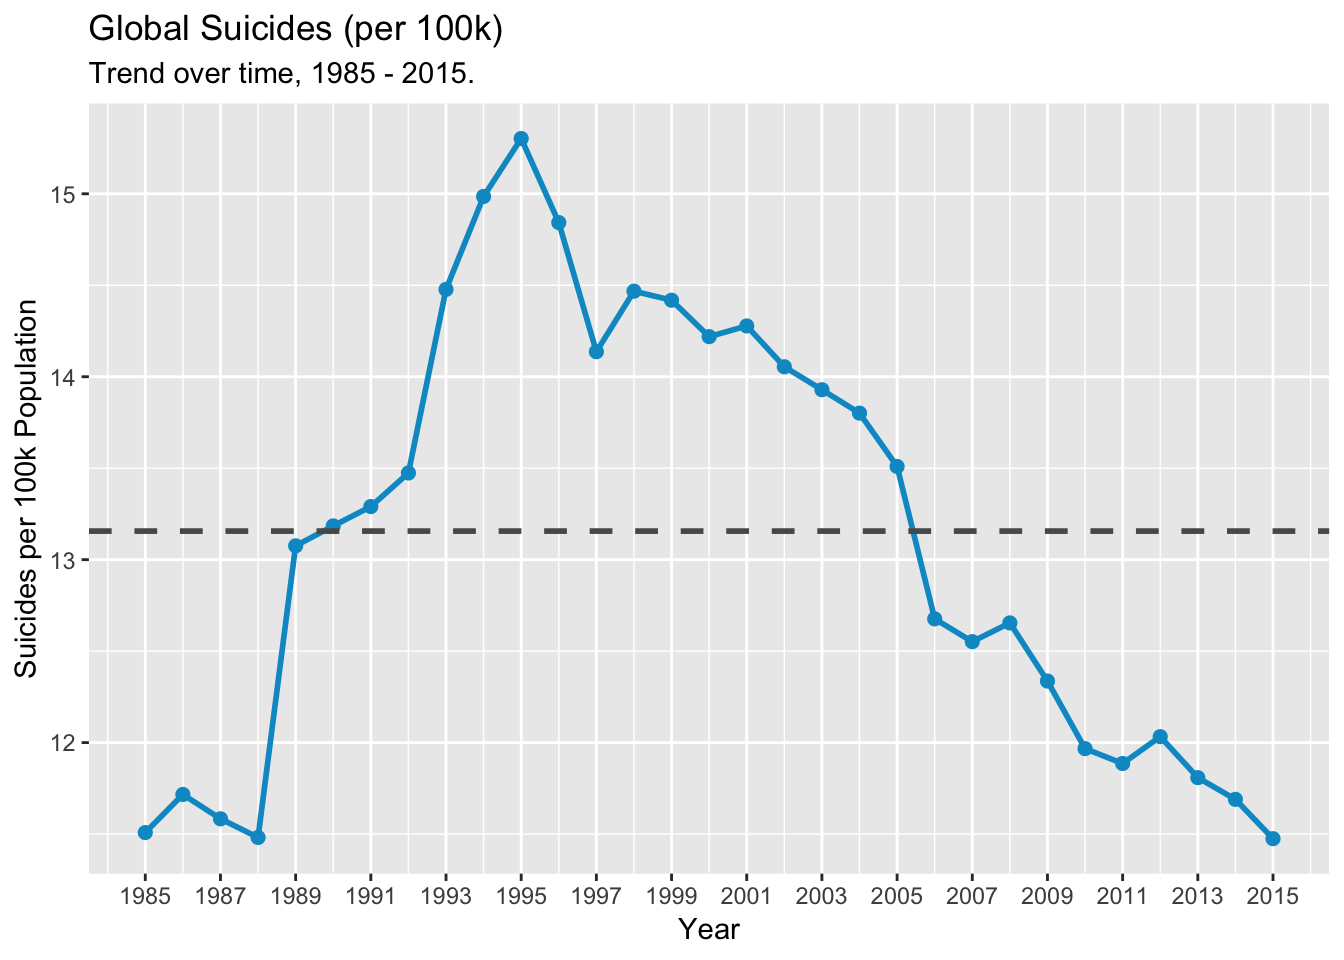
\includegraphics{suicides_files/figure-latex/unnamed-chunk-2-1.pdf}
\emph{Abbildung 1: Suicides per 100k per Year. Gestrichelte Linie ist
der globale Durchschnitt.}

\hypertarget{selbstmorde-nach-kontinent}{%
\subsubsection{Selbstmorde nach
Kontinent}\label{selbstmorde-nach-kontinent}}

\begin{Shaded}
\begin{Highlighting}[]
\NormalTok{continent <-}\StringTok{ }\NormalTok{data }\OperatorTok
\StringTok{  }\KeywordTok{group_by}\NormalTok{(continent) }\OperatorTok
\StringTok{  }\KeywordTok{summarize}\NormalTok{(}\DataTypeTok{suicide_per_100k =}\NormalTok{ (}\KeywordTok{sum}\NormalTok{(}\KeywordTok{as.numeric}\NormalTok{(suicides_no)) }\OperatorTok{/}\StringTok{ }\KeywordTok{sum}\NormalTok{(}\KeywordTok{as.numeric}\NormalTok{(population))) }\OperatorTok{*}\StringTok{ }\DecValTok{100000}\NormalTok{) }\OperatorTok
\StringTok{  }\KeywordTok{arrange}\NormalTok{(suicide_per_100k)}

\NormalTok{continent}\OperatorTok{$}\NormalTok{continent <-}\StringTok{ }\KeywordTok{factor}\NormalTok{(continent}\OperatorTok{$}\NormalTok{continent, }\DataTypeTok{ordered =}\NormalTok{ T, }\DataTypeTok{levels =}\NormalTok{ continent}\OperatorTok{$}\NormalTok{continent)}

\NormalTok{continent_plot <-}\StringTok{ }\KeywordTok{ggplot}\NormalTok{(continent, }\KeywordTok{aes}\NormalTok{(}\DataTypeTok{x =}\NormalTok{ continent, }\DataTypeTok{y =}\NormalTok{ suicide_per_100k, }\DataTypeTok{fill =}\NormalTok{ continent)) }\OperatorTok{+}\StringTok{ }
\StringTok{  }\KeywordTok{geom_bar}\NormalTok{(}\DataTypeTok{stat =} \StringTok{"identity"}\NormalTok{) }\OperatorTok{+}\StringTok{ }
\StringTok{  }\KeywordTok{labs}\NormalTok{(}\DataTypeTok{title =} \StringTok{"Global Suicides (per 100k), by Continent"}\NormalTok{,}
  \DataTypeTok{x =} \StringTok{"Continent"}\NormalTok{, }
  \DataTypeTok{y =} \StringTok{"Suicides per 100k"}\NormalTok{, }
  \DataTypeTok{fill =} \StringTok{"Continent"}\NormalTok{) }\OperatorTok{+}
\StringTok{  }\KeywordTok{theme}\NormalTok{(}\DataTypeTok{legend.position =} \StringTok{"none"}\NormalTok{, }\DataTypeTok{title =} \KeywordTok{element_text}\NormalTok{(}\DataTypeTok{size =} \DecValTok{10}\NormalTok{)) }\OperatorTok{+}\StringTok{ }
\StringTok{  }\KeywordTok{scale_y_continuous}\NormalTok{(}\DataTypeTok{breaks =} \KeywordTok{seq}\NormalTok{(}\DecValTok{0}\NormalTok{, }\DecValTok{20}\NormalTok{, }\DecValTok{1}\NormalTok{), }\DataTypeTok{minor_breaks =}\NormalTok{ F)}

\NormalTok{continent_time <-}\StringTok{ }\NormalTok{data }\OperatorTok
\StringTok{  }\KeywordTok{group_by}\NormalTok{(year, continent) }\OperatorTok
\StringTok{  }\KeywordTok{summarize}\NormalTok{(}\DataTypeTok{suicide_per_100k =}\NormalTok{ (}\KeywordTok{sum}\NormalTok{(}\KeywordTok{as.numeric}\NormalTok{(suicides_no)) }\OperatorTok{/}\StringTok{ }\KeywordTok{sum}\NormalTok{(}\KeywordTok{as.numeric}\NormalTok{(population))) }\OperatorTok{*}\StringTok{ }\DecValTok{100000}\NormalTok{)}

\NormalTok{continent_time}\OperatorTok{$}\NormalTok{continent <-}\StringTok{ }\KeywordTok{factor}\NormalTok{(continent_time}\OperatorTok{$}\NormalTok{continent, }\DataTypeTok{ordered =}\NormalTok{ T, }\DataTypeTok{levels =}\NormalTok{ continent}\OperatorTok{$}\NormalTok{continent)}

\NormalTok{continent_time_plot <-}\StringTok{ }\KeywordTok{ggplot}\NormalTok{(continent_time, }\KeywordTok{aes}\NormalTok{(}\DataTypeTok{x =}\NormalTok{ year, }\DataTypeTok{y =}\NormalTok{ suicide_per_100k, }\DataTypeTok{col =} \KeywordTok{factor}\NormalTok{(continent))) }\OperatorTok{+}\StringTok{ }
\StringTok{  }\KeywordTok{facet_grid}\NormalTok{(continent }\OperatorTok{~}\StringTok{ }\NormalTok{., }\DataTypeTok{scales =} \StringTok{"free_y"}\NormalTok{) }\OperatorTok{+}\StringTok{ }
\StringTok{  }\KeywordTok{geom_line}\NormalTok{() }\OperatorTok{+}\StringTok{ }
\StringTok{  }\KeywordTok{geom_point}\NormalTok{() }\OperatorTok{+}\StringTok{ }
\StringTok{  }\KeywordTok{labs}\NormalTok{(}\DataTypeTok{title =} \StringTok{"Trends Over Time, by Continent"}\NormalTok{, }
       \DataTypeTok{x =} \StringTok{"Year"}\NormalTok{, }
       \DataTypeTok{y =} \StringTok{"Suicides per 100k"}\NormalTok{, }
       \DataTypeTok{color =} \StringTok{"Continent"}\NormalTok{) }\OperatorTok{+}\StringTok{ }
\StringTok{  }\KeywordTok{theme}\NormalTok{(}\DataTypeTok{legend.position =} \StringTok{"none"}\NormalTok{, }\DataTypeTok{title =} \KeywordTok{element_text}\NormalTok{(}\DataTypeTok{size =} \DecValTok{10}\NormalTok{)) }\OperatorTok{+}\StringTok{ }
\StringTok{  }\KeywordTok{scale_x_continuous}\NormalTok{(}\DataTypeTok{breaks =} \KeywordTok{seq}\NormalTok{(}\DecValTok{1985}\NormalTok{, }\DecValTok{2015}\NormalTok{, }\DecValTok{5}\NormalTok{), }\DataTypeTok{minor_breaks =}\NormalTok{ F)}

\NormalTok{continent_plot}
\end{Highlighting}
\end{Shaded}

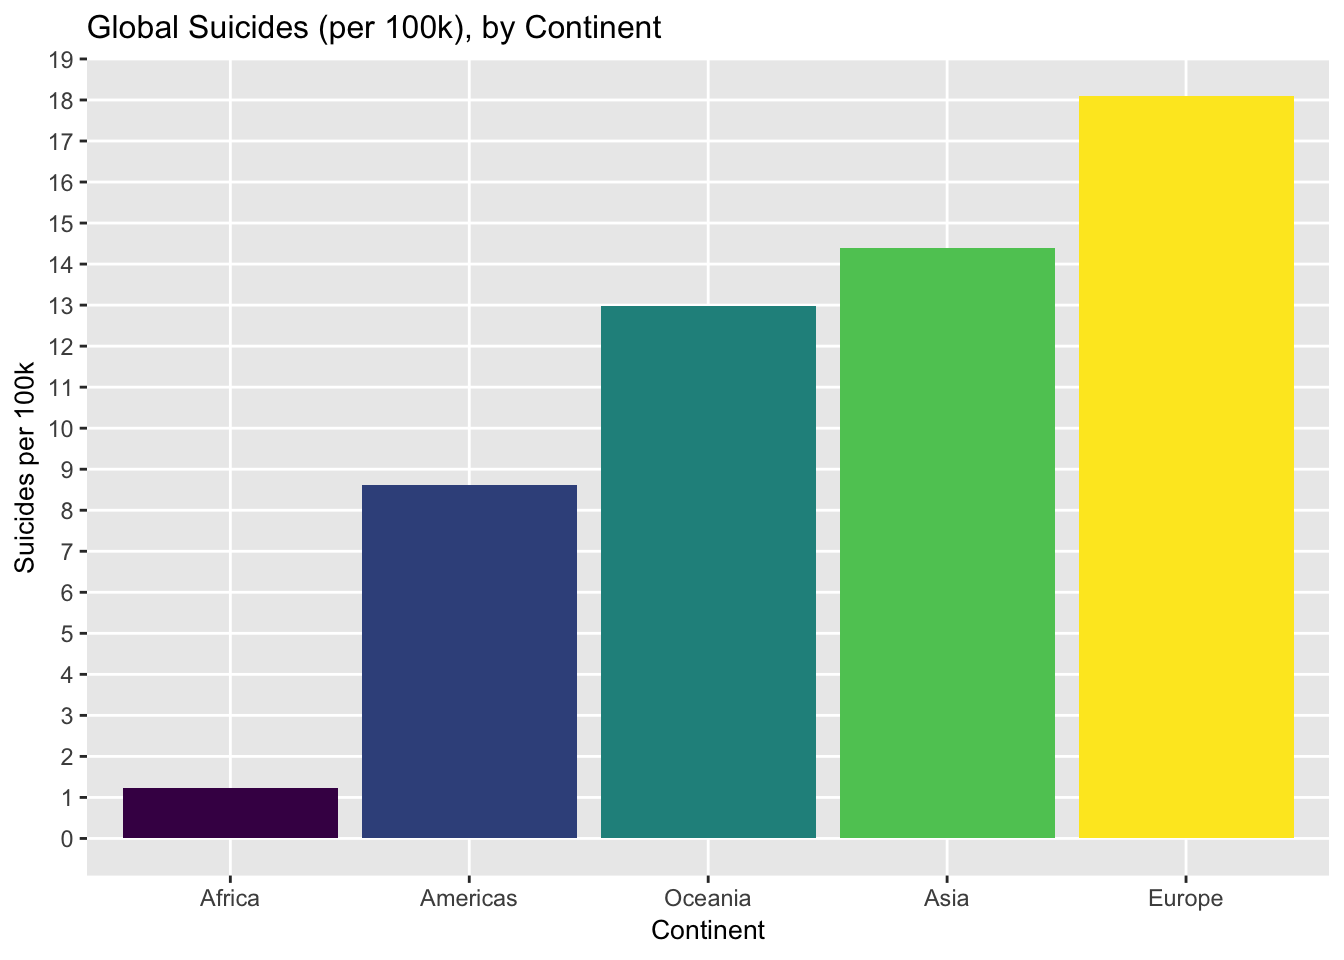
\includegraphics{suicides_files/figure-latex/unnamed-chunk-3-1.pdf}

\begin{Shaded}
\begin{Highlighting}[]
\NormalTok{continent_time_plot}
\end{Highlighting}
\end{Shaded}

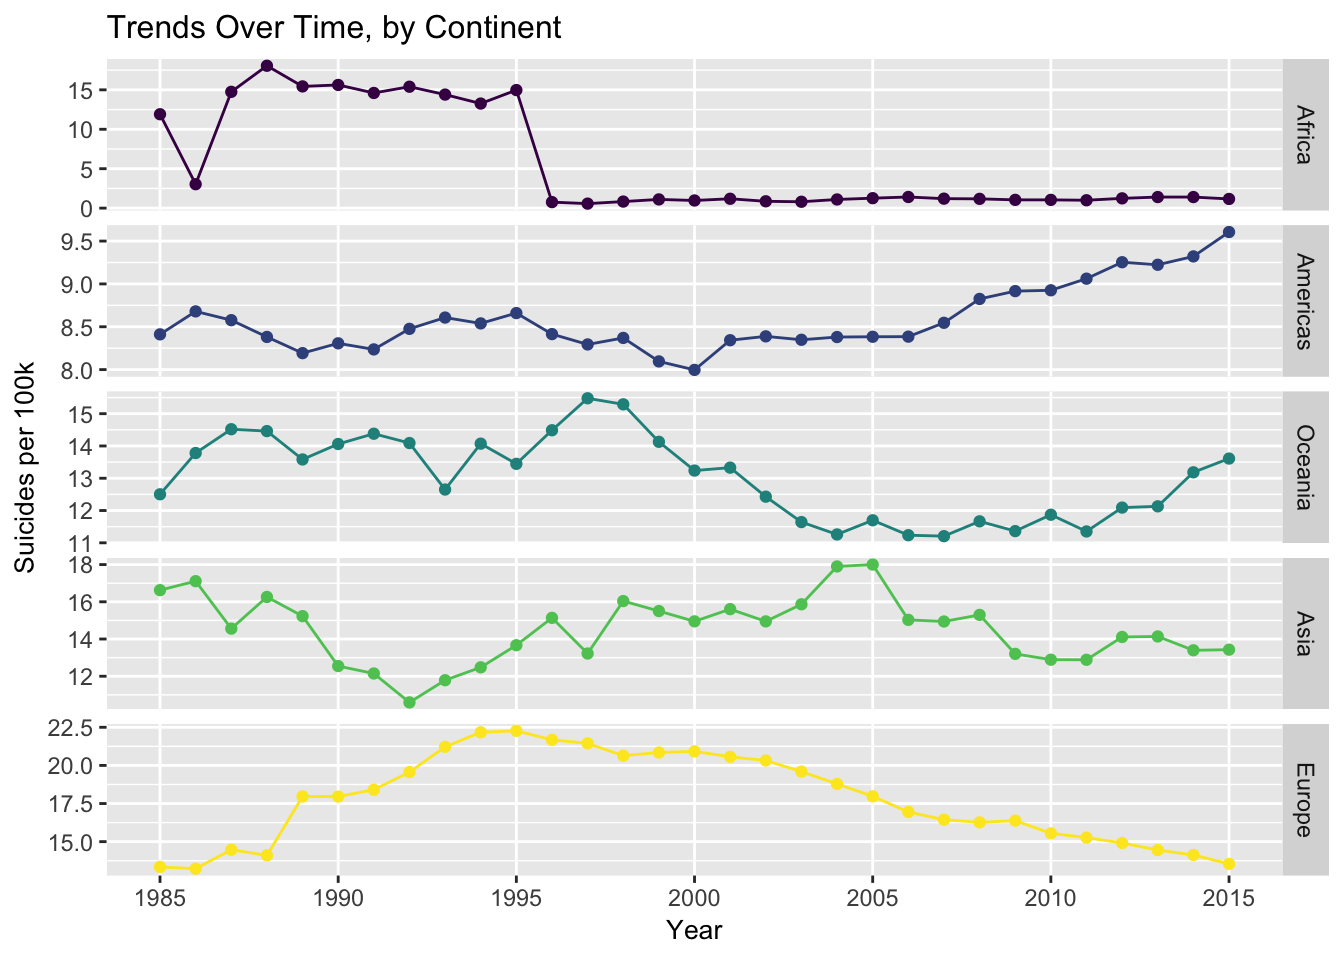
\includegraphics{suicides_files/figure-latex/unnamed-chunk-4-1.pdf}

\hypertarget{selbstmorde-nach-geschlecht}{%
\subsubsection{Selbstmorde nach
Geschlecht}\label{selbstmorde-nach-geschlecht}}

\begin{Shaded}
\begin{Highlighting}[]
\NormalTok{sex_plot <-}\StringTok{ }\NormalTok{data }\OperatorTok
\StringTok{  }\KeywordTok{group_by}\NormalTok{(sex) }\OperatorTok
\StringTok{  }\KeywordTok{summarize}\NormalTok{(}\DataTypeTok{suicide_per_100k =}\NormalTok{ (}\KeywordTok{sum}\NormalTok{(}\KeywordTok{as.numeric}\NormalTok{(suicides_no)) }\OperatorTok{/}\StringTok{ }\KeywordTok{sum}\NormalTok{(}\KeywordTok{as.numeric}\NormalTok{(population))) }\OperatorTok{*}\StringTok{ }\DecValTok{100000}\NormalTok{) }\OperatorTok
\KeywordTok{ggplot}\NormalTok{(}\KeywordTok{aes}\NormalTok{(}\DataTypeTok{x =}\NormalTok{ sex, }\DataTypeTok{y =}\NormalTok{ suicide_per_100k, }\DataTypeTok{fill =}\NormalTok{ sex)) }\OperatorTok{+}
\StringTok{  }\KeywordTok{geom_bar}\NormalTok{(}\DataTypeTok{stat =} \StringTok{"identity"}\NormalTok{) }\OperatorTok{+}\StringTok{ }
\StringTok{  }\KeywordTok{labs}\NormalTok{(}\DataTypeTok{title =} \StringTok{"Global suicides (per 100k), by Sex"}\NormalTok{,}
       \DataTypeTok{x =} \StringTok{"Sex"}\NormalTok{, }
       \DataTypeTok{y =} \StringTok{"Suicides per 100k"}\NormalTok{) }\OperatorTok{+}
\StringTok{  }\KeywordTok{theme}\NormalTok{(}\DataTypeTok{legend.position =} \StringTok{"none"}\NormalTok{) }\OperatorTok{+}\StringTok{ }
\StringTok{  }\KeywordTok{scale_y_continuous}\NormalTok{(}\DataTypeTok{breaks =} \KeywordTok{seq}\NormalTok{(}\DecValTok{0}\NormalTok{, }\DecValTok{25}\NormalTok{), }\DataTypeTok{minor_breaks =}\NormalTok{ F)}


\NormalTok{sex_time_plot <-}\StringTok{ }\NormalTok{data }\OperatorTok
\StringTok{  }\KeywordTok{group_by}\NormalTok{(year, sex) }\OperatorTok
\StringTok{  }\KeywordTok{summarize}\NormalTok{(}\DataTypeTok{suicide_per_100k =}\NormalTok{ (}\KeywordTok{sum}\NormalTok{(}\KeywordTok{as.numeric}\NormalTok{(suicides_no)) }\OperatorTok{/}\StringTok{ }\KeywordTok{sum}\NormalTok{(}\KeywordTok{as.numeric}\NormalTok{(population))) }\OperatorTok{*}\StringTok{ }\DecValTok{100000}\NormalTok{) }\OperatorTok
\StringTok{  }\KeywordTok{ggplot}\NormalTok{(}\KeywordTok{aes}\NormalTok{(}\DataTypeTok{x =}\NormalTok{ year, }\DataTypeTok{y =}\NormalTok{ suicide_per_100k, }\DataTypeTok{col =} \KeywordTok{factor}\NormalTok{(sex))) }\OperatorTok{+}\StringTok{ }
\StringTok{  }\KeywordTok{facet_grid}\NormalTok{(sex }\OperatorTok{~}\StringTok{ }\NormalTok{., }\DataTypeTok{scales =} \StringTok{"free_y"}\NormalTok{) }\OperatorTok{+}\StringTok{ }
\StringTok{  }\KeywordTok{geom_line}\NormalTok{() }\OperatorTok{+}\StringTok{ }
\StringTok{  }\KeywordTok{geom_point}\NormalTok{() }\OperatorTok{+}\StringTok{ }
\StringTok{  }\KeywordTok{labs}\NormalTok{(}\DataTypeTok{title =} \StringTok{"Trends Over Time, by Sex"}\NormalTok{, }
       \DataTypeTok{x =} \StringTok{"Year"}\NormalTok{, }
       \DataTypeTok{y =} \StringTok{"Suicides per 100k"}\NormalTok{, }
       \DataTypeTok{color =} \StringTok{"Sex"}\NormalTok{) }\OperatorTok{+}\StringTok{ }
\StringTok{  }\KeywordTok{theme}\NormalTok{(}\DataTypeTok{legend.position =} \StringTok{"none"}\NormalTok{) }\OperatorTok{+}\StringTok{ }
\StringTok{  }\KeywordTok{scale_x_continuous}\NormalTok{(}\DataTypeTok{breaks =} \KeywordTok{seq}\NormalTok{(}\DecValTok{1985}\NormalTok{, }\DecValTok{2015}\NormalTok{, }\DecValTok{5}\NormalTok{), }\DataTypeTok{minor_breaks =}\NormalTok{ F)}

\NormalTok{sex_plot}
\end{Highlighting}
\end{Shaded}

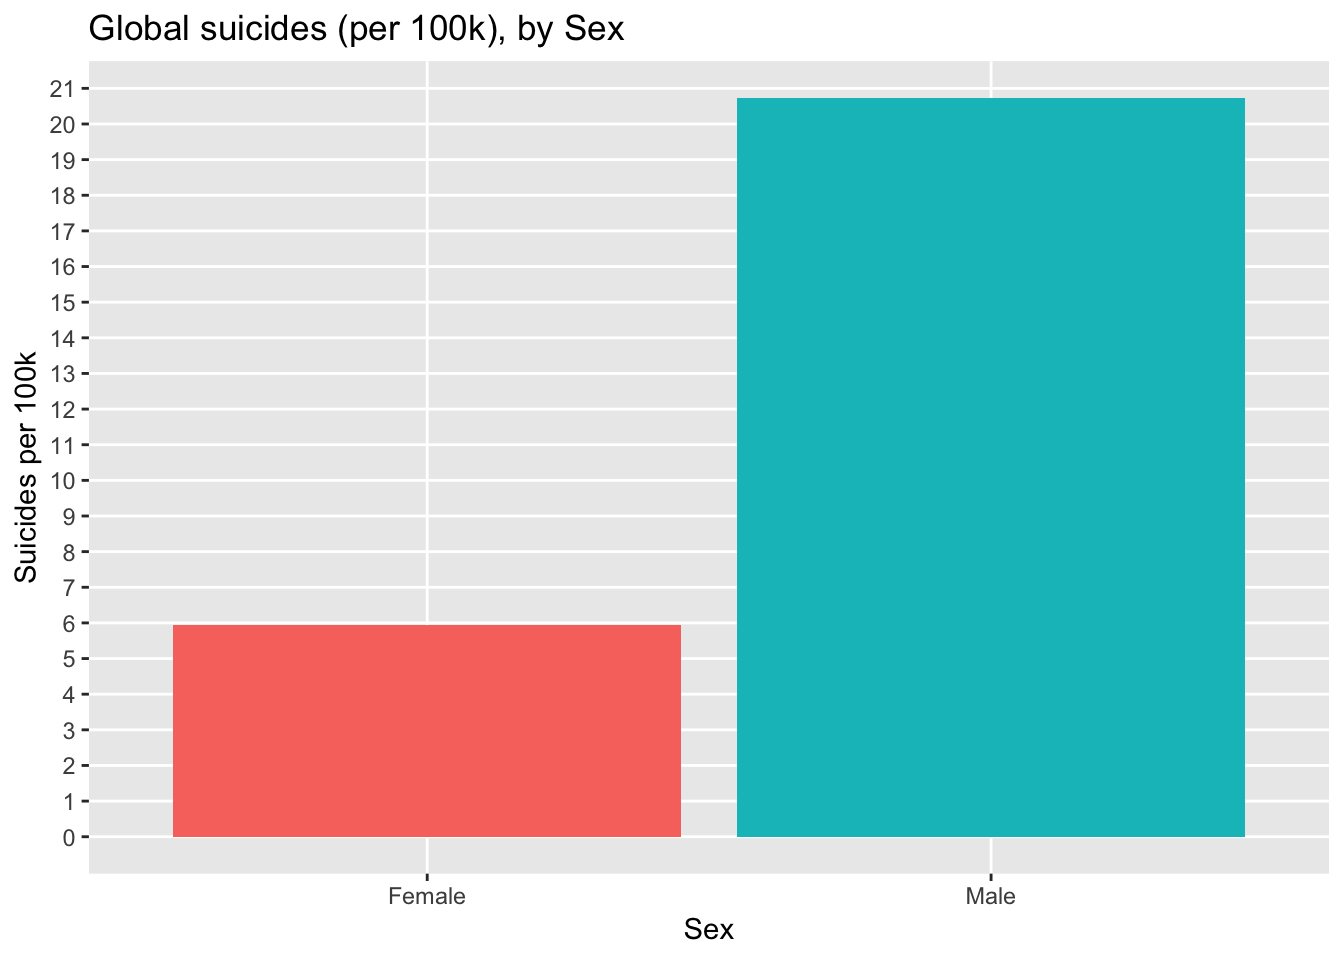
\includegraphics{suicides_files/figure-latex/unnamed-chunk-5-1.pdf}

\begin{Shaded}
\begin{Highlighting}[]
\NormalTok{sex_time_plot}
\end{Highlighting}
\end{Shaded}

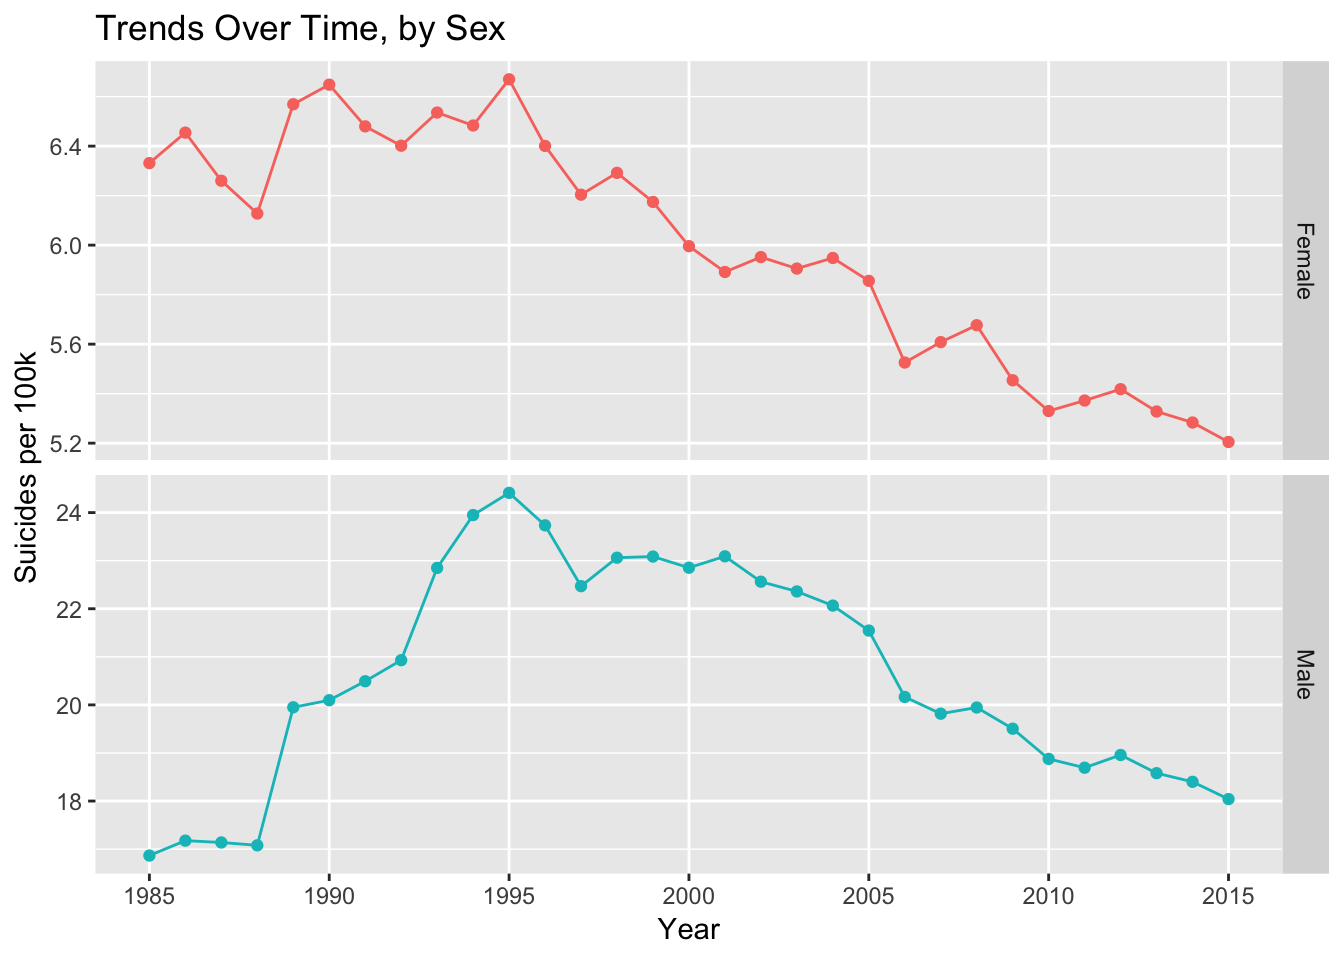
\includegraphics{suicides_files/figure-latex/unnamed-chunk-6-1.pdf}

\hypertarget{selbstmorde-nach-country}{%
\subsubsection{Selbstmorde nach
Country}\label{selbstmorde-nach-country}}

\begin{Shaded}
\begin{Highlighting}[]
\CommentTok{# mit "fig.width = 10, fig.height = 13" erreichen wir, dass das Bild richtig angezeigt wird und nicht zu klein ist}
\NormalTok{country <-}\StringTok{ }\NormalTok{data }\OperatorTok
\StringTok{  }\KeywordTok{group_by}\NormalTok{(country, continent) }\OperatorTok
\StringTok{  }\KeywordTok{summarize}\NormalTok{(}\DataTypeTok{n =} \KeywordTok{n}\NormalTok{(), }
            \DataTypeTok{suicide_per_100k =}\NormalTok{ (}\KeywordTok{sum}\NormalTok{(}\KeywordTok{as.numeric}\NormalTok{(suicides_no)) }\OperatorTok{/}\StringTok{ }\KeywordTok{sum}\NormalTok{(}\KeywordTok{as.numeric}\NormalTok{(population))) }\OperatorTok{*}\StringTok{ }\DecValTok{100000}\NormalTok{) }\OperatorTok
\StringTok{  }\KeywordTok{arrange}\NormalTok{(}\KeywordTok{desc}\NormalTok{(suicide_per_100k))}

\NormalTok{country}\OperatorTok{$}\NormalTok{country <-}\StringTok{ }\KeywordTok{factor}\NormalTok{(country}\OperatorTok{$}\NormalTok{country, }
                          \DataTypeTok{ordered =}\NormalTok{ T, }
                          \DataTypeTok{levels =} \KeywordTok{rev}\NormalTok{(country}\OperatorTok{$}\NormalTok{country))}

\KeywordTok{ggplot}\NormalTok{(country, }\KeywordTok{aes}\NormalTok{(}\DataTypeTok{x =}\NormalTok{ country, }\DataTypeTok{y =}\NormalTok{ suicide_per_100k, }\DataTypeTok{fill =}\NormalTok{ continent)) }\OperatorTok{+}\StringTok{ }
\StringTok{  }\KeywordTok{geom_bar}\NormalTok{(}\DataTypeTok{stat =} \StringTok{"identity"}\NormalTok{) }\OperatorTok{+}\StringTok{ }
\StringTok{  }\KeywordTok{geom_hline}\NormalTok{(}\DataTypeTok{yintercept =}\NormalTok{ global_average, }\DataTypeTok{linetype =} \DecValTok{2}\NormalTok{, }\DataTypeTok{color =} \StringTok{"grey35"}\NormalTok{, }\DataTypeTok{size =} \FloatTok{0.6}\NormalTok{) }\OperatorTok{+}
\StringTok{  }\KeywordTok{labs}\NormalTok{(}\DataTypeTok{title =} \StringTok{"Global suicides per 100k, by Country"}\NormalTok{,}
       \DataTypeTok{x =} \StringTok{"Country"}\NormalTok{, }
       \DataTypeTok{y =} \StringTok{"Suicides per 100k"}\NormalTok{, }
       \DataTypeTok{fill =} \StringTok{"Continent"}\NormalTok{) }\OperatorTok{+}
\StringTok{  }\KeywordTok{coord_flip}\NormalTok{() }\OperatorTok{+}\StringTok{ }\CommentTok{#Achsen drehen, weil sont Land nicht zu lesen ist}
\StringTok{  }\KeywordTok{scale_y_continuous}\NormalTok{(}\DataTypeTok{breaks =} \KeywordTok{seq}\NormalTok{(}\DecValTok{0}\NormalTok{, }\DecValTok{45}\NormalTok{, }\DecValTok{2}\NormalTok{)) }\OperatorTok{+}
\StringTok{  }\KeywordTok{scale_x_discrete}\NormalTok{(}\StringTok{"Country"}\NormalTok{, }\DataTypeTok{labels =}\NormalTok{  , }\DataTypeTok{position =} \StringTok{"bottom"}\NormalTok{) }\OperatorTok{+}
\StringTok{  }\KeywordTok{theme}\NormalTok{(}\DataTypeTok{legend.position =} \StringTok{"bottom"}\NormalTok{)}
\end{Highlighting}
\end{Shaded}

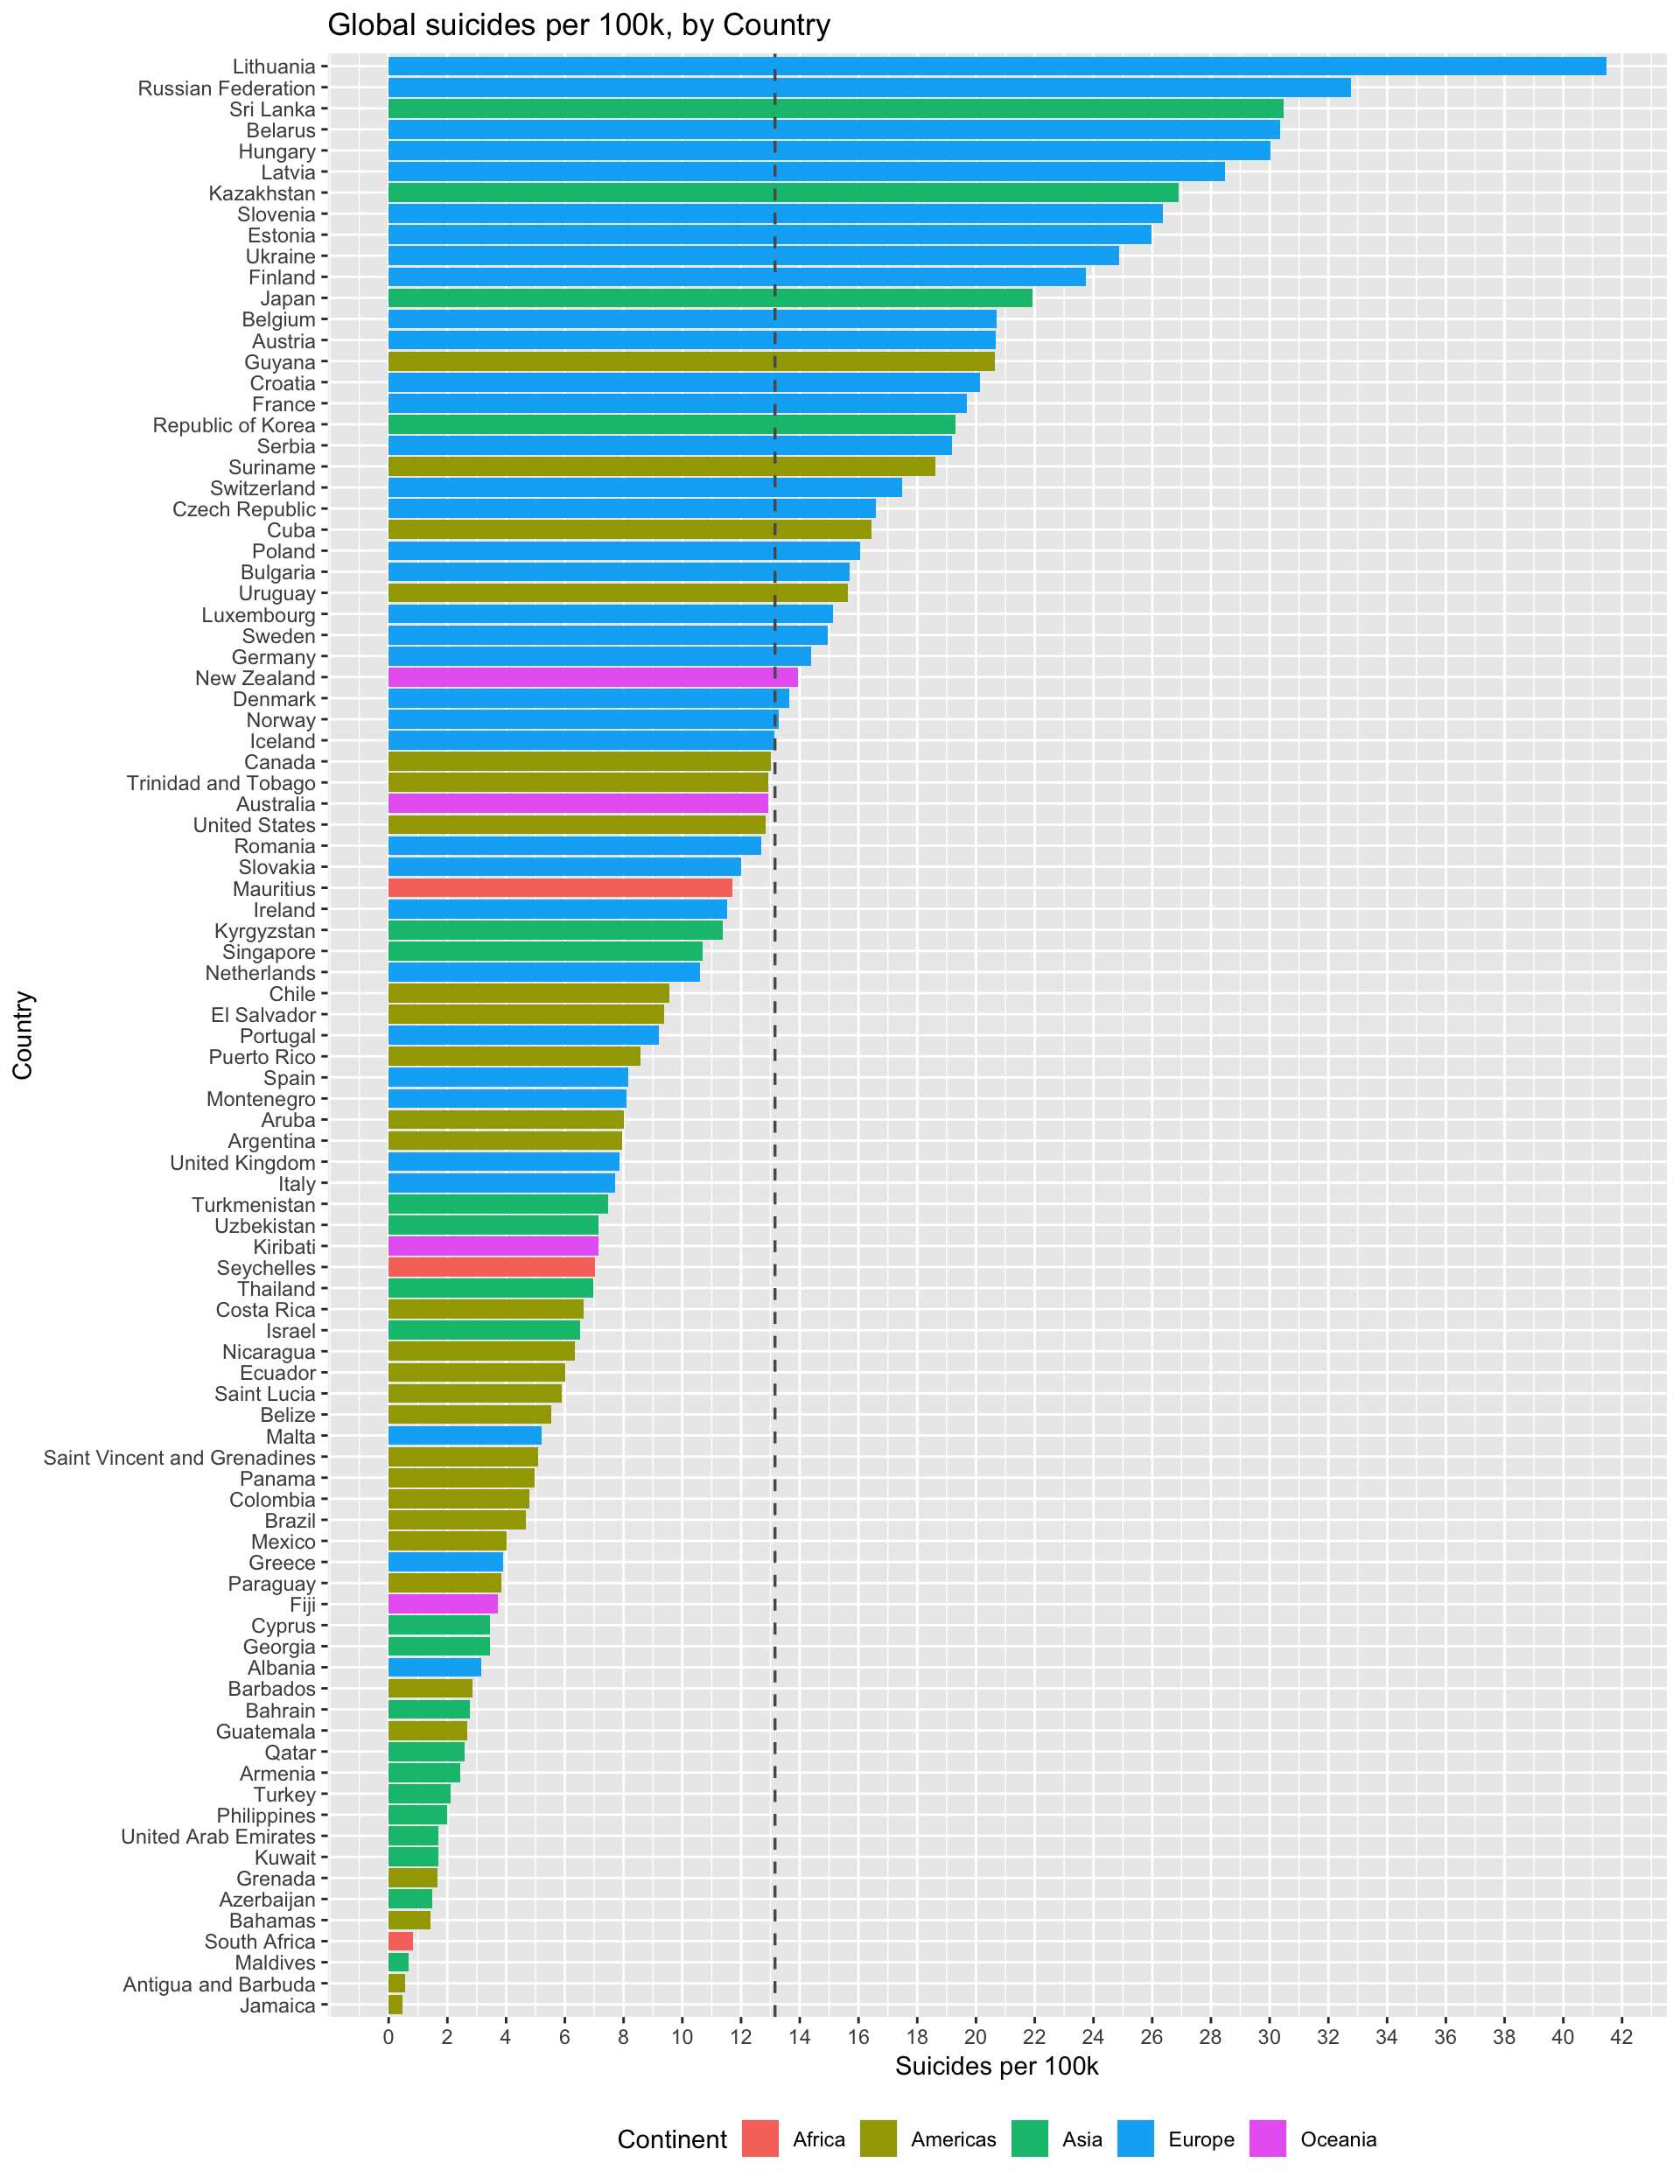
\includegraphics{suicides_files/figure-latex/unnamed-chunk-7-1.pdf}


\end{document}
